% This is samplepaper.tex, a sample chapter demonstrating the
% LLNCS macro package for Springer Computer Science proceedings;
% Version 2.20 of 2017/10/04
%
\documentclass[runningheads]{llncs}
%
\makeatletter
\usepackage[algoruled,boxed,lined]{algorithm2e}
\makeatletter
\g@addto@macro{\@algocf@init}{\SetKwInOut{Parameter}{Parameters}}
\makeatother
\usepackage{amsmath}
\usepackage{amssymb}

\numberwithin{equation}{subsection} % numbers on equations

% \usepackage{graphicx}\usepackage{draftwatermark}
% \SetWatermarkText{\textsc{Draft}}

% -------------------- My Packages -------------------- %
\usepackage{hyperref}
\usepackage{xcolor}
\usepackage[utf8]{inputenc}
\usepackage{csquotes}

\usepackage{fontspec}
% \setmonofont{Roboto Mono} % sadly, does not look good
\usepackage{minted}

% Draw neural network
\usepackage{tikz}

\usepackage{fancyref}
\let\oldfref\fref
\renewcommand{\fref}[1]{[\oldfref{#1}]}

% \raggedbottom % add to allow whitespace on end of pages and not evenly distribute text

%---------- Ich bin ein verdammter Künstler ----------
\usepackage{listings}
\definecolor{maroon}{RGB}{128, 0, 0}
\definecolor{pinegreen}{RGB}{1, 121, 111}
\definecolor{darkmidnightblue}{RGB}{0, 51, 102}
\definecolor{rwthblue}{RGB}{0, 84, 159}
% www.colorhexa.com for color references

% Quiet Light
\definecolor{background}{HTML}{f5f5f5}
\definecolor{keyword}{HTML}{4b83cd}
\definecolor{constant}{HTML}{ab6526}
\definecolor{function}{HTML}{aa3731} % bold
\definecolor{comment}{HTML}{aaaaaa} % italic
\definecolor{string}{HTML}{448c27}

% ---------- Hyperref -----------
\hypersetup{colorlinks=true,
            breaklinks=true,
            urlcolor=rwthblue,
            linkcolor=rwthblue,
            citecolor=rwthblue}
\def\UrlBreaks{\do\/\do-}
% -------------------------------

\newcommand{\fat}[1]{\mathbf{#1}}
\DeclareMathOperator*{\argmax}{arg\,max}
\DeclareMathOperator*{\argmin}{arg\,min}

% ------------------ End My Packages ------------------ %

% Used for displaying a sample figure. If possible, figure files should
% be included in EPS format.
%
% If you use the hyperref package, please uncomment the following line
% to display URLs in blue roman font according to Springer's eBook style:
% \renewcommand\UrlFont{\color{blue}\rmfamily}
% I don't really care.
\renewcommand\UrlFont{\rmfamily}


\begin{document}
%
\title{Back-Propagation and Algorithms for Training Artificial Neural Networks}
%
\titlerunning{Back-Propagation and Algorithms for Training Artificial Neural Networks}
% If the paper title is too long for the running head, you can set
% an abbreviated paper title here
%
\author{Gero F. Kauerauf}
%
\authorrunning{Kauerauf}
% First names are abbreviated in the running head.
% If there are more than two authors, 'et al.' is used.
%
\institute{RWTH Aachen University\\ \email{gero.kauerauf@rwth-aachen.de}} 
%
\maketitle              % typeset the header of the contribution
%
\begin{abstract}
    In this paper, we elaborate on the key concepts in training neural networks.
    First of all, we explain the fundamentals of feedforward networks.
    We then consider basic algorithms such as back-propagation and stochastic gradient descent, which are widely used for training.
    Besides, we illustrate important details with examples and use graphics when necessary.
    The result is a compact overview of standard methods.
\keywords{Deep Learning \and Back-Propagation \and Stochastic Gradient Descent \and Feedforward Networks}
\end{abstract}
%
%
%

% Introduction
% Section - Introduction
\section{Introduction}
\label{sec:introduction}

In this paper, we elaborate on the main algorithms used for training neural networks.
We especially lay focus on \emph{feedforward networks} and \emph{supervised learing}, for which we describe these algorithms in great detail.
For better understanding, this paper itself is structured in the same order the algorithms and methods to train are used in.
Key elements are:
\begin{itemize}
    \item Structure of \emph{feedforward networks} and \emph{forward propagation}
    \item \emph{Cost functions} and \emph{computational graphs} for these networks
    \item \emph{Backward-propagation}
    \item \emph{Stochastic gradient descent}
\end{itemize}
We make use of examples and graphics at key points for better understanding.
Furthermore, we have simplified unnecessary complex practical parts, that are not essential for a fundamental understanding.
This paper is mostly based on the standard textbook by \textbf{Goodfellow et al.} \cite{Goodfellow-et-al-2016}.

% Section - Problem Description
\section{Problem description}
\label{sec:problem-description}

Since computers are still getting better every year, one would expect that we could solve more and more problems.
This may be true in some fields, however, there are still problems that are very hard to solve.

This class is filled with problems that are hard to describe mathematically.
Take for example a image of a \emph{cat} and a \emph{dog}.
A human can intuitively recognize a cat on an image and is able with ease to distinguish between those two animals.
However up to this day, it is not possible to describe the key characteristics of a \emph{cat} mathematically,
so that one can build an algorithm that solves this problem.

Another class of problems is the ones that can be described perfectly but are simply too complicated.
These are for example games like chess.
We have no problem with describing the rules of chess.
However, due to the sheer amount of possible moves and positions in chess, we have trouble analyzing games perfectly.
Theoretically, writing an algorithm that \enquote{brute-forces} a game of chess is no problem, but practically this algorithm is too slow.
Even worse, computers might never be fast enough!

This is where \emph{neural networks} come into play.
For these kinds of problems, they are the best we currently have.

% Introduction to Feedforward Networks
% Section - Feedforward networks
\section{Feedforward Networks}
\emph{Deep feedforward networks}, also called \emph{feedforward neural networks} or \emph{multilayer perceptrons} (MLPs) are are basic deep learning models.
Their main purpose is to approximate some kind of function \(f^*(x)\).
Take for example a classification function \(y = f^*(x)\), where every input \(x\) maps to a class \(y\).
A feedforward network now aims to learn the best parameters \(\Theta\) for a function \(y = f(x, \Theta)\) that approximates \(f^*(x)\).

These models are \emph{networks} due to the fact that they can be represented by \emph{directed graphs}.
One of those \emph{graphs} models the consecutive execution of functions whose composition is \(f\).
They are called \emph{feedforward networks} because the input \(x\) flows through these functions without any \emph{feedback} connections.
This means that the graph is \emph{acyclic}.
If the graph is \emph{not acyclic} and therefore \(feedback\) connections exist, we speak of \emph{recurrent neural networks}.

For example let \(f(x) = (f^3 \circ f^2 \circ f^1)(x) = f^3(f^2(f^1(x)))\).
We now define the \emph{depth} of a \emph{feedforward network} \(f\) as the number of functions that compose it.
Our example has a \emph{depth} of \(3\).
These kind of chains are very typical in \emph{neural networks}, as each function in the chain represents a layer in the \emph{directed acyclic graph}.
The last element of the chain (in our example \(f^1\)) and therefore the last layer in the graph is called the \emph{output layer} as it maps the input \(x\) to its final value.
If we think of \(f\) as a classifier function the elements of the \emph{codomain} of \(f^1\) are the classes.
Likewise, the elements of the \emph{domain} of the first function in the chain (in our example \(f^3\)) are the inputs of the network.
The first layer is called \emph{input layer}.
Layers between the \emph{input} and \emph{output} layer are called \emph{hidden layers}.

\subsection{Feedforward network graphs}
As proposed earlier we can also think of \emph{neural networks} as \emph{acyclic directed graphs}.
Loosely inspired by neuroscience, \emph{neurons} are interpreted as \emph{nodes} and \emph{synapses} as \emph{edges}.
Each \emph{node} now receives input from an arbitrary amount of neurons in the previous layer and computes an output with its own activation function.
An \emph{edges} on the other hand has a scalar \emph{weight}.
These \emph{weights} are now what can be adjusted to changed the output of the neural network.

It is shown that in most feedforward networks a \emph{rectifier linear units} (reLU) (\(f(x) = \text{max}(0, x)\)) activation function works best. \cite{Nair-Hinton} \cite{inproceedings}
However, in certain cases other activation functions might perform better.
Such would be for example the \emph{swish} activation function (\(f(x) = x * \text{sigmoid}(x)\)), that tends to perform better than reLU on deeper models. \cite{DBLP:journals/corr/abs-1710-05941}

% Small sample neural network graph
\begin{figure}[h]
    \centering
    \label{fig:dnn-example}
    
    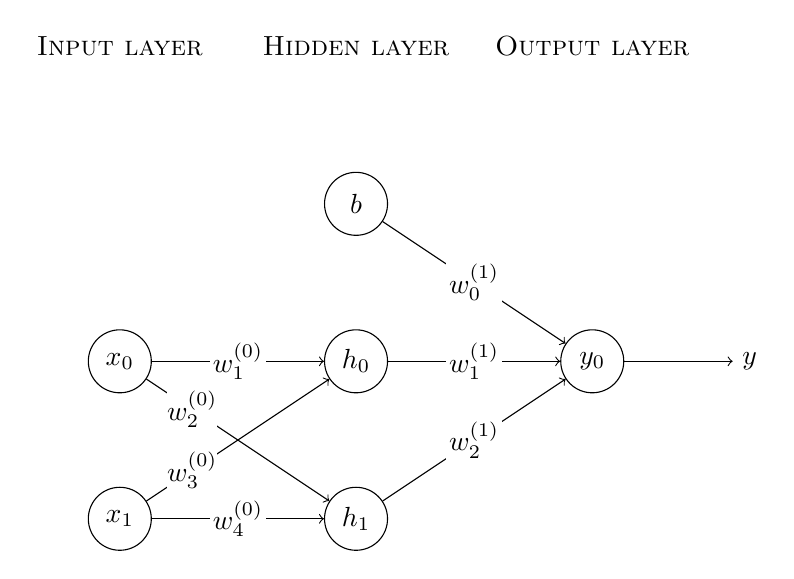
\begin{tikzpicture}
        \def\vert{2}
        \def\hori{3}
        \tikzstyle{place}=[circle, draw=black, minimum size=8mm]
        \tikzstyle{label}=[inner sep=1pt, fill=white]
        
        % Input
        \draw node at (0 * \hori, 4 * \vert) [black, ] {\textsc{Input layer}};
        
        \draw node at (0 * \hori, 2 * \vert) [place] (input_0) {$x_0$};	
        \draw node at (0 * \hori, 1 * \vert) [place] (input_1) {$x_1$};
        
        
        % Hidden
        \draw node at (1 * \hori, 4 * \vert) [black, ] {\textsc{Hidden layer}};
        
        \draw node at (1 * \hori, 3 * \vert) [place] (hidden_0) {$b$};
        \draw node at (1 * \hori, 2 * \vert) [place] (hidden_1) {$h_0$};	
        \draw node at (1 * \hori, 1 * \vert) [place] (hidden_2) {$h_1$};	
        
        % Output
        \draw node at (2 * \hori, 4 * \vert) [black, ] {\textsc{Output layer}};
        
        \draw node at (2 * \hori, 2 * \vert) [place] (output_0) {$y_0$};
        
        % Out
        \node at (8, 2 * \vert) [black, ] (out_0) {$y$};
		
        % Input -> Hidden
        % \foreach \i in {0,...,1}
        %  	 \foreach \j in {1,...,2}
        %		 \draw [->] (input_\i) to node[near start, below] {$w_{\i}^{(0)}$} (hidden_\j);
        \draw [->] (input_0) to node[label] {$w_{1}^{(0)}$} (hidden_1);
        \draw [->] (input_0) to node[label, near start, inner sep=0pt] {$w_{2}^{(0)}$} (hidden_2);
        \draw [->] (input_1) to node[label, near start, inner sep=0pt] {$w_{3}^{(0)}$} (hidden_1);
        \draw [->] (input_1) to node[label] {$w_{4}^{(0)}$} (hidden_2);
        
        
        % Hidden -> Output
        \foreach \i in {0,...,2}
		\foreach \j in {0,...,0}
        \draw [->] (hidden_\i) to node[label] {$w_{\i}^{(1)}$} (output_\j);
        
        \foreach \i in {0,...,0}
		\draw [->] (output_\i) to (out_\i);
        
    \end{tikzpicture}
    \caption{Example DNN with a single hidden layer}
\end{figure}

This DNN \fref{fig:dnn-example} can now also be described by its \emph{weight matrices}. 

We can represent the weights of the edges between two layers as a \emph{weight matrices} \(\fat{W} \in \mathbb{R}^{m \times n}\).
The input can be represented as a vector \({x \in \mathbb{R}^n}\).
Calculating the output of a neural network can therefore be achieved by iterative \emph{matrix-vector multiplication} and component-wise usage of the activation function on each layer.

For \fref{fig:dnn-example} the weight matrices are
\begin{equation}
    \fat{W}^{(0)} =
    \begin{pmatrix}
        w_{2}^{(0)} & w_{4}^{(0)} \\
        w_{3}^{(0)} & w_{5}^{(0)}
    \end{pmatrix}, \quad
    \fat{W}^{(1)} = 
    \begin{pmatrix}
        w_{1}^{(1)} & w_{2}^{(1)}
    \end{pmatrix}.
\end{equation}
With the corresponding bias vectors
\begin{equation}
    b^{(0)} =
    \begin{pmatrix}
        w_{0}^{(0)} \\
        w_{1}^{(0)}
    \end{pmatrix}, \quad
    b^{(1)} =
    \begin{pmatrix}
        w_{0}^{(1)}
    \end{pmatrix}.
\end{equation}
In order to get more \enquote{flexible} we add a \emph{bias} node to each layer.
This bias node always has an input of \(1\) and describes the constant in a linear equation.

Let \(f(x)\) now be the activation function and
\begin{equation}
    x =
    \begin{pmatrix}
        x_0 \\
        x_1
    \end{pmatrix},
\end{equation}
the input vector.
The output vector for \fref{fig:dnn-example} can be calculated by evaluating the following equations.
\begin{equation}
    x_0 =
    f(W^{(0)}x + b^{0}) =
    f(
    \begin{pmatrix}
        w_{2}^{(0)} & w_{4}^{(0)} \\
        w_{3}^{(0)} & w_{5}^{(0)}
    \end{pmatrix}
    \begin{pmatrix}
        x_0 \\
        x_1å
    \end{pmatrix}
    +
    \begin{pmatrix}
        w_{0}^{(0)} \\
        w_{1}^{(0)}
    \end{pmatrix}
    )
\end{equation}
\begin{equation}
    y =
    f(W^{(1)}x_0 + b^{1}) =
    f(
    \begin{pmatrix}
        w_{1}^{(1)} & w_{2}^{(1)}
    \end{pmatrix}
    x_0
    +
    \begin{pmatrix}
        w_{0}^{(1)}
    \end{pmatrix}
    )
\end{equation}
Where the activation function \(f\) is used component-wise.

% \subsection{tf.keras.Sequential}

% Introduction to Deep Learning
% Section - Deep learning
\section{Deep learning}
\label{sec:deep-learning}

\emph{Deep learning} refers to the broader family of machine learning algorithms, that are based on artificial neural networks.
Feedforward networks fall into the family of \emph{deep neural networks} (DNNs).

The typical procedure when training a feedforward network is to define a \emph{cost function} for it.
The \emph{cost function} is dependent on the \emph{weights} of the neural network and describes the \emph{error} of the network.
Remember, for a given input \(\fat{x}\) the network computes the output \(\hat{\fat{y}}\).
The cost function now measures the distance of \(\hat{\fat{y}}\) to the real \(\fat{y}\), this distance is called the \emph{error}.
In the context of \emph{supervised learning}, we know \(\fat{y}\), because a human has previously \enquote{classified} the input.
A minimum in the \emph{cost function} therefore minimizes the \emph{error} of the network.
In order to minimize the \emph{cost function} we have to compute its gradient and then \emph{adjust} the weights.
The computation of the gradient is performed by the \emph{back-propagation algorithm}.
The \emph{adjustment} is then performed by an \emph{optimizing algorithm}.

% Subsection - Cost Functions
\subsection{Cost Functions}
A very important aspect of neural networks is the choice of a cost function.
In most cases we can make use of \emph{maximum likelihood} principle, because a neural network defines a distribution \(p(y \vert x ; \theta)\).xw

% Subsection - Computational Graphs
\subsection{Computational graphs}

Another important concept is the one of \emph{computational graphs}.
A \emph{computational graph} describes a mathematical expression.
Such a \emph{directed graph} consists out of nodes and edges.
A node represents an arbitrary variable, that may be a scalar, a vector, a matrix or of any other type.
Then there are also \emph{operations}.
An \emph{operation} can be informally described as a label on a node.
This label defines the operation that is performed on the input.
Whereas the input is given by the \emph{directed edges} to that node.
An operation can take an arbitrary amount of inputs and stores the result in its node.

An example is given by \fref{fig:comp-graph-example}.

\begin{figure}[h]
    \centering
    \label{fig:comp-graph-example}
    
    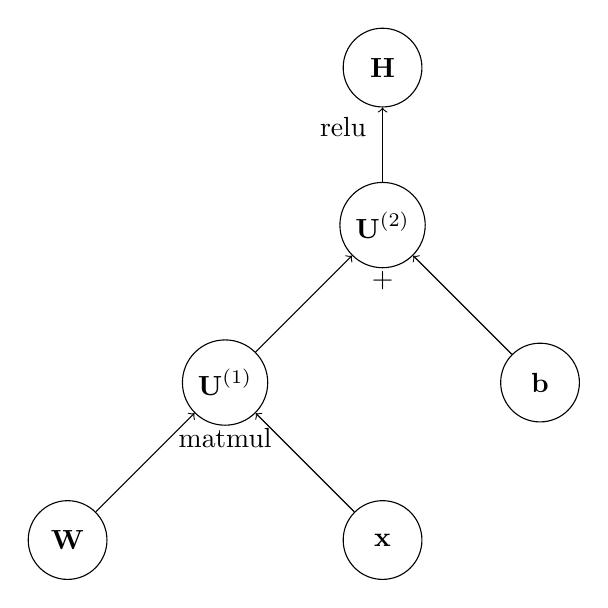
\begin{tikzpicture}
        \def\vert{2}
        \def\hori{2}
        \tikzstyle{place}=[circle, draw=black, minimum size=10mm]
        
        % Nodes
        \node[place] (w) at (0 * \hori, 0 * \vert) {\textbf{W}};
        \node[place] (x) at (2 * \hori, 0 * \vert) {\textbf{x}};
        
        \node[place, label={[shift={(0.0,-1.5)}]{\text{matmul}}}] (u1) at (1 * \hori, 1 * \vert) {$\textbf{U}^{(1)}$};
        \node[place] (b) at (3 * \hori, 1 * \vert) {\textbf{b}};
        
        
        \node[place, label={[shift={(0.0,-1.5)}]{\text{+}}}] (u2) at (2 * \hori, 2 * \vert) {$\textbf{U}^{(2)}$};
        
        \node[place, label={[shift={(-0.5,-1.5)}]{\text{relu}}}] (h) at (2 * \hori, 3 * \vert) {\textbf{H}};
        
        % Edges
        \draw [->] (w) to (u1);
        \draw [->] (x) to (u1);

        \draw [->] (u1) to (u2);
        \draw [->] (b) to (u2);
        
        \draw [->] (u2) to (h);
        
    \end{tikzpicture}
    \caption{Example of a computational graph}
\end{figure}

% Subsection - Back-Propagation
\subsection{Back-Propagation}
\label{sec:back-propagation}

Often mistaken for the whole learning algorithm, 
back-propagation just refers to the algorithm for computing the gradient of a computational graph.
It is called back-propagation because we evaluate the gradient for the output layer backwards to the input layer.
In some way it can be understood as a counter part to the forward propagation.
As already discussed, forward propagation describes the process of calculating the output \(\hat{\fat{y}}\) of a feedforward network for a given input \(\fat{x}\).
Back-propagation on the other hand now works it way from the output layer to the input layer in order to compute the gradient for a given input \(\fat{x}\), a calculated output \(\hat{\fat{y}}\) and
a \enquote{wanted} output \(\fat{y}\).

A common misbelief, is that the back-propagation is performed on the feedforward network itself, whereas it is rather done on the computational graph of the cost function.
Optimizing the \emph{weights} in the graph of the cost function also optimizes them in the network!
Since the back-propagation only computes the gradient, the \enquote{real} learning is performed by an \emph{optimizing} algorithm, such as \emph{stochastic gradient descent} \fref{sec:stochastic-gradient-descent}.

\paragraph{Chain Rule of Calculus.}
The chain rule of calculus describes how to calculate the derivative of a function that is composed of other functions.
Let \(f: \mathbb{R} \rightarrow \mathbb{R}\) and \(g: \mathbb{R} \rightarrow \mathbb{R}\) both be differentiable.
If \(y = g(x)\) and \(z = f(y) = f(g(x))\), then
\begin{equation}
    \frac{\partial z}{\partial x} = \frac{\partial z}{\partial y} \frac{\partial y}{\partial x}.
\end{equation}
This can of course also be written as
\begin{equation}
    (f(g(x)))^\prime = f^\prime (g(x)) g^\prime(x).
\end{equation}
This can now be extended to arbitrary dimension.
Let \(g: \mathbb{R}^m \rightarrow \mathbb{R}^n\) and \(f: \mathbb{R}^n \rightarrow \mathbb{R}\).
If \(\fat{y} = g(\fat{x})\) and \(z = f(g(\fat{x})) = f(\fat{y})\), then
\begin{equation}
    \frac{\partial z}{\partial \fat{x}_{i}} = \sum_{j} \frac{\partial z}{\partial \fat{y}_{j}} \frac{\partial \fat{y}_{j}}{\partial \fat{x}_{i}}.
\end{equation}
Using the \(\nabla\) operator for the gradient, this can also be written as
\begin{equation}
    \label{eq:jacobian-vector-product}
    \nabla_{\fat{x}} z = \bigg( \frac{\partial \fat{y}}{\fat{x}} \bigg)^{T} \nabla_{\fat{y}} z,
\end{equation}
where \(\frac{\partial \fat{y}}{\partial x}\) is the \(n \times m\) Jacobian of \(g\).
Since feedforward networks often work with tensors of arbitrary dimension and not vectors, we would have to change our notation a bit in order to deal with them.
We would simply \enquote{flatten} the tensor and use multiple coordinates as indices for the dimensions.
However I am not going to introduce this here, since the concept can already be understood with vectors. \\

The general idea of the back-propagation algorithm is simple.
If we want to compute the gradient of \(z\) with respect to \(x\) we start at the node \(z\).
We observe that the gradient of \(z\) with respect to \(z\) is \(1\), since \(\frac{\partial z}{\partial z} = 1\).
We then compute the gradient with respect to each parent of \(z\) by multiplying the current gradient by the Jacobian that produced \(z\).
This means we propagate backwards through the network by multiplying with Jacobians until we reach \(x\).
If there are multiple paths, we simply take them each after another.

More formally this means that each node in the computational graph corresponds to a variable (in our case a vector).
Each variable \(\fat{v}\) has now the following subroutines:
\begin{itemize}
    \item \texttt{operation(\(\fat{v}\))}, gets the mathematical operation that defines \(\fat{v}\),
    which is represented by the edges flowing into \(\fat{v}\) and the relation, e.g. matrix multiplication
    \item \texttt{children(\(\fat{v}\))}, returns an array that contains the variables that are children of \(\fat{v}\) in the graph
    \item \texttt{parents(\(\fat{v}\))}, returns an array that contains the variables that are parents of \(\fat{v}\) in the graph 
\end{itemize}
Furthermore every operation \texttt{op} is associated with a \texttt{back\_prop} operation, that computes the product described by \fref{eq:jacobian-vector-product}.
Let \(\fat{C} = \fat{AB}\), and the gradient of a scalar \(z\) with respect to \(\fat{C}\) be \(\fat{g} \in \mathbb{R}^n\).
Then \texttt{back\_prop} has to define the gradient of matrix multiplication for \(\fat{A}\) and \(\fat{B}\).
This means that \texttt{op.back\_prop(parents(..), \(\fat{A}\), \(\fat{g}\))} evaluates to \(\fat{g}\fat{B}^T \in \mathbb{R}^n\), because \(\frac{\partial \fat{C}}{\partial \fat{A}} = \fat{B}^T\).
Analogously, the call of \texttt{op.back\_prop(parents(..), \(\fat{B}\), \(\fat{g}\))} evaluates to \(\fat{A}^T\fat{g} \in \mathbb{R}^n\).
Formally the call of \texttt{op.back\_prop(parents(..), \(\fat{V}\), \(\fat{g}\))} returns
\begin{equation}
    \sum_{i} \big( \nabla_{\fat{V}} \texttt{op.f(parents(..))}_{i} \fat{G}_{i} \big),
\end{equation}
where \texttt{op.f} is the mathematical relation (e.g. matrix multiplication).
The two dots in the call of the \texttt{parent(..)} function refer to the current node we are at.
It is of great importance that \texttt{op.back\_prop} always pretends that all of its inputs are distinct.
Take for example the function \(x^2\) the \texttt{back\_prop} should now for both inputs return \(x\).
It will later add those two \(x\) together to receive the correct derivate of \(2x\).

By making use of the \texttt{back\_prop} function like this, we receive a very general back-propagation algorithm.


% Subsection - Stochastic gradient descent
\subsection{Stochastic gradient descent}

% \subsection{tf.model}

% Section - State of the Art
\section{State of the art}
\label{sec:state-of-the-art}

Modern neural network implementations such as Keras in TensorFlow \cite{tensorflow2015-whitepaper} are used in a broad variety of fields.
Research interest in neural networks has been on a rise for the last 40 years and it seems like this trend is not going to stop anytime soon.
With computers getting constantly faster and new different types of neural networks coming up, the number of fields in which neural networks are used also increases.

Especially in the last years, there has been a huge interest and development in convolutional neural network.
Modern optimization algorithms such as \emph{Ftrl} \cite{McMahan} and new activation functions like \emph{swish} \cite{DBLP:journals/corr/abs-1710-05941} by Google are increasing the performance of them even more.

% Section - Conclusion
\section{Conclusion}
\label{sec:conclusion}

%
% ---- Bibliography ----
%
% BibTeX users should specify bibliography style 'splncs04'.
% References will then be sorted and formatted in the correct style.
%
\bibliographystyle{splncs04}
\bibliography{refs}

\end{document}
